\documentclass[twoside]{book}

% Packages required by doxygen
\usepackage{fixltx2e}
\usepackage{calc}
\usepackage{doxygen}
\usepackage[export]{adjustbox} % also loads graphicx
\usepackage{graphicx}
\usepackage[utf8]{inputenc}
\usepackage{makeidx}
\usepackage{multicol}
\usepackage{multirow}
\PassOptionsToPackage{warn}{textcomp}
\usepackage{textcomp}
\usepackage[nointegrals]{wasysym}
\usepackage[table]{xcolor}

% Font selection
\usepackage[T1]{fontenc}
\usepackage[scaled=.90]{helvet}
\usepackage{courier}
\usepackage{amssymb}
\usepackage{sectsty}
\renewcommand{\familydefault}{\sfdefault}
\allsectionsfont{%
  \fontseries{bc}\selectfont%
  \color{darkgray}%
}
\renewcommand{\DoxyLabelFont}{%
  \fontseries{bc}\selectfont%
  \color{darkgray}%
}
\newcommand{\+}{\discretionary{\mbox{\scriptsize$\hookleftarrow$}}{}{}}

% Page & text layout
\usepackage{geometry}
\geometry{%
  a4paper,%
  top=2.5cm,%
  bottom=2.5cm,%
  left=2.5cm,%
  right=2.5cm%
}
\tolerance=750
\hfuzz=15pt
\hbadness=750
\setlength{\emergencystretch}{15pt}
\setlength{\parindent}{0cm}
\setlength{\parskip}{3ex plus 2ex minus 2ex}
\makeatletter
\renewcommand{\paragraph}{%
  \@startsection{paragraph}{4}{0ex}{-1.0ex}{1.0ex}{%
    \normalfont\normalsize\bfseries\SS@parafont%
  }%
}
\renewcommand{\subparagraph}{%
  \@startsection{subparagraph}{5}{0ex}{-1.0ex}{1.0ex}{%
    \normalfont\normalsize\bfseries\SS@subparafont%
  }%
}
\makeatother

% Headers & footers
\usepackage{fancyhdr}
\pagestyle{fancyplain}
\fancyhead[LE]{\fancyplain{}{\bfseries\thepage}}
\fancyhead[CE]{\fancyplain{}{}}
\fancyhead[RE]{\fancyplain{}{\bfseries\leftmark}}
\fancyhead[LO]{\fancyplain{}{\bfseries\rightmark}}
\fancyhead[CO]{\fancyplain{}{}}
\fancyhead[RO]{\fancyplain{}{\bfseries\thepage}}
\fancyfoot[LE]{\fancyplain{}{}}
\fancyfoot[CE]{\fancyplain{}{}}
\fancyfoot[RE]{\fancyplain{}{\bfseries\scriptsize Generated by Doxygen }}
\fancyfoot[LO]{\fancyplain{}{\bfseries\scriptsize Generated by Doxygen }}
\fancyfoot[CO]{\fancyplain{}{}}
\fancyfoot[RO]{\fancyplain{}{}}
\renewcommand{\footrulewidth}{0.4pt}
\renewcommand{\chaptermark}[1]{%
  \markboth{#1}{}%
}
\renewcommand{\sectionmark}[1]{%
  \markright{\thesection\ #1}%
}

% Indices & bibliography
\usepackage{natbib}
\usepackage[titles]{tocloft}
\setcounter{tocdepth}{3}
\setcounter{secnumdepth}{5}
\makeindex

% Hyperlinks (required, but should be loaded last)
\usepackage{ifpdf}
\ifpdf
  \usepackage[pdftex,pagebackref=true]{hyperref}
\else
  \usepackage[ps2pdf,pagebackref=true]{hyperref}
\fi
\hypersetup{%
  colorlinks=true,%
  linkcolor=blue,%
  citecolor=blue,%
  unicode%
}

% Custom commands
\newcommand{\clearemptydoublepage}{%
  \newpage{\pagestyle{empty}\cleardoublepage}%
}

\usepackage{caption}
\captionsetup{labelsep=space,justification=centering,font={bf},singlelinecheck=off,skip=4pt,position=top}

%===== C O N T E N T S =====

\begin{document}

% Titlepage & ToC
\hypersetup{pageanchor=false,
             bookmarksnumbered=true,
             pdfencoding=unicode
            }
\pagenumbering{alph}
\begin{titlepage}
\vspace*{7cm}
\begin{center}%
{\Large opdracht\+\_\+3\+\_\+1 }\\
\vspace*{1cm}
{\large Generated by Doxygen 1.8.13}\\
\end{center}
\end{titlepage}
\clearemptydoublepage
\pagenumbering{roman}
\tableofcontents
\clearemptydoublepage
\pagenumbering{arabic}
\hypersetup{pageanchor=true}

%--- Begin generated contents ---
\chapter{Hierarchical Index}
\section{Class Hierarchy}
This inheritance list is sorted roughly, but not completely, alphabetically\+:\begin{DoxyCompactList}
\item \contentsline{section}{drawable}{\pageref{classdrawable}}{}
\begin{DoxyCompactList}
\item \contentsline{section}{circle}{\pageref{classcircle}}{}
\begin{DoxyCompactList}
\item \contentsline{section}{ball}{\pageref{classball}}{}
\end{DoxyCompactList}
\item \contentsline{section}{line}{\pageref{classline}}{}
\item \contentsline{section}{rectangle}{\pageref{classrectangle}}{}
\begin{DoxyCompactList}
\item \contentsline{section}{wall}{\pageref{classwall}}{}
\end{DoxyCompactList}
\end{DoxyCompactList}
\item \contentsline{section}{vector}{\pageref{classvector}}{}
\item \contentsline{section}{window}{\pageref{classwindow}}{}
\end{DoxyCompactList}

\chapter{Class Index}
\section{Class List}
Here are the classes, structs, unions and interfaces with brief descriptions\+:\begin{DoxyCompactList}
\item\contentsline{section}{\hyperlink{classball}{ball} }{\pageref{classball}}{}
\item\contentsline{section}{\hyperlink{classcircle}{circle} }{\pageref{classcircle}}{}
\item\contentsline{section}{\hyperlink{classdrawable}{drawable} }{\pageref{classdrawable}}{}
\item\contentsline{section}{\hyperlink{classline}{line} }{\pageref{classline}}{}
\item\contentsline{section}{\hyperlink{classrectangle}{rectangle} }{\pageref{classrectangle}}{}
\item\contentsline{section}{\hyperlink{classvector}{vector} }{\pageref{classvector}}{}
\item\contentsline{section}{\hyperlink{classwall}{wall} \\*Wall }{\pageref{classwall}}{}
\item\contentsline{section}{\hyperlink{classwindow}{window} }{\pageref{classwindow}}{}
\end{DoxyCompactList}

\chapter{File Index}
\section{File List}
Here is a list of all documented files with brief descriptions\+:\begin{DoxyCompactList}
\item\contentsline{section}{{\bfseries ball.\+hpp} }{\pageref{ball_8hpp}}{}
\item\contentsline{section}{{\bfseries circle.\+hpp} }{\pageref{circle_8hpp}}{}
\item\contentsline{section}{{\bfseries drawable.\+hpp} }{\pageref{drawable_8hpp}}{}
\item\contentsline{section}{{\bfseries line.\+hpp} }{\pageref{line_8hpp}}{}
\item\contentsline{section}{{\bfseries rectangle.\+hpp} }{\pageref{rectangle_8hpp}}{}
\item\contentsline{section}{{\bfseries vector.\+hpp} }{\pageref{vector_8hpp}}{}
\item\contentsline{section}{\hyperlink{wall_8hpp}{wall.\+hpp} }{\pageref{wall_8hpp}}{}
\item\contentsline{section}{{\bfseries window.\+hpp} }{\pageref{window_8hpp}}{}
\end{DoxyCompactList}

\chapter{Class Documentation}
\hypertarget{classball}{}\section{ball Class Reference}
\label{classball}\index{ball@{ball}}
Inheritance diagram for ball\+:\begin{figure}[H]
\begin{center}
\leavevmode
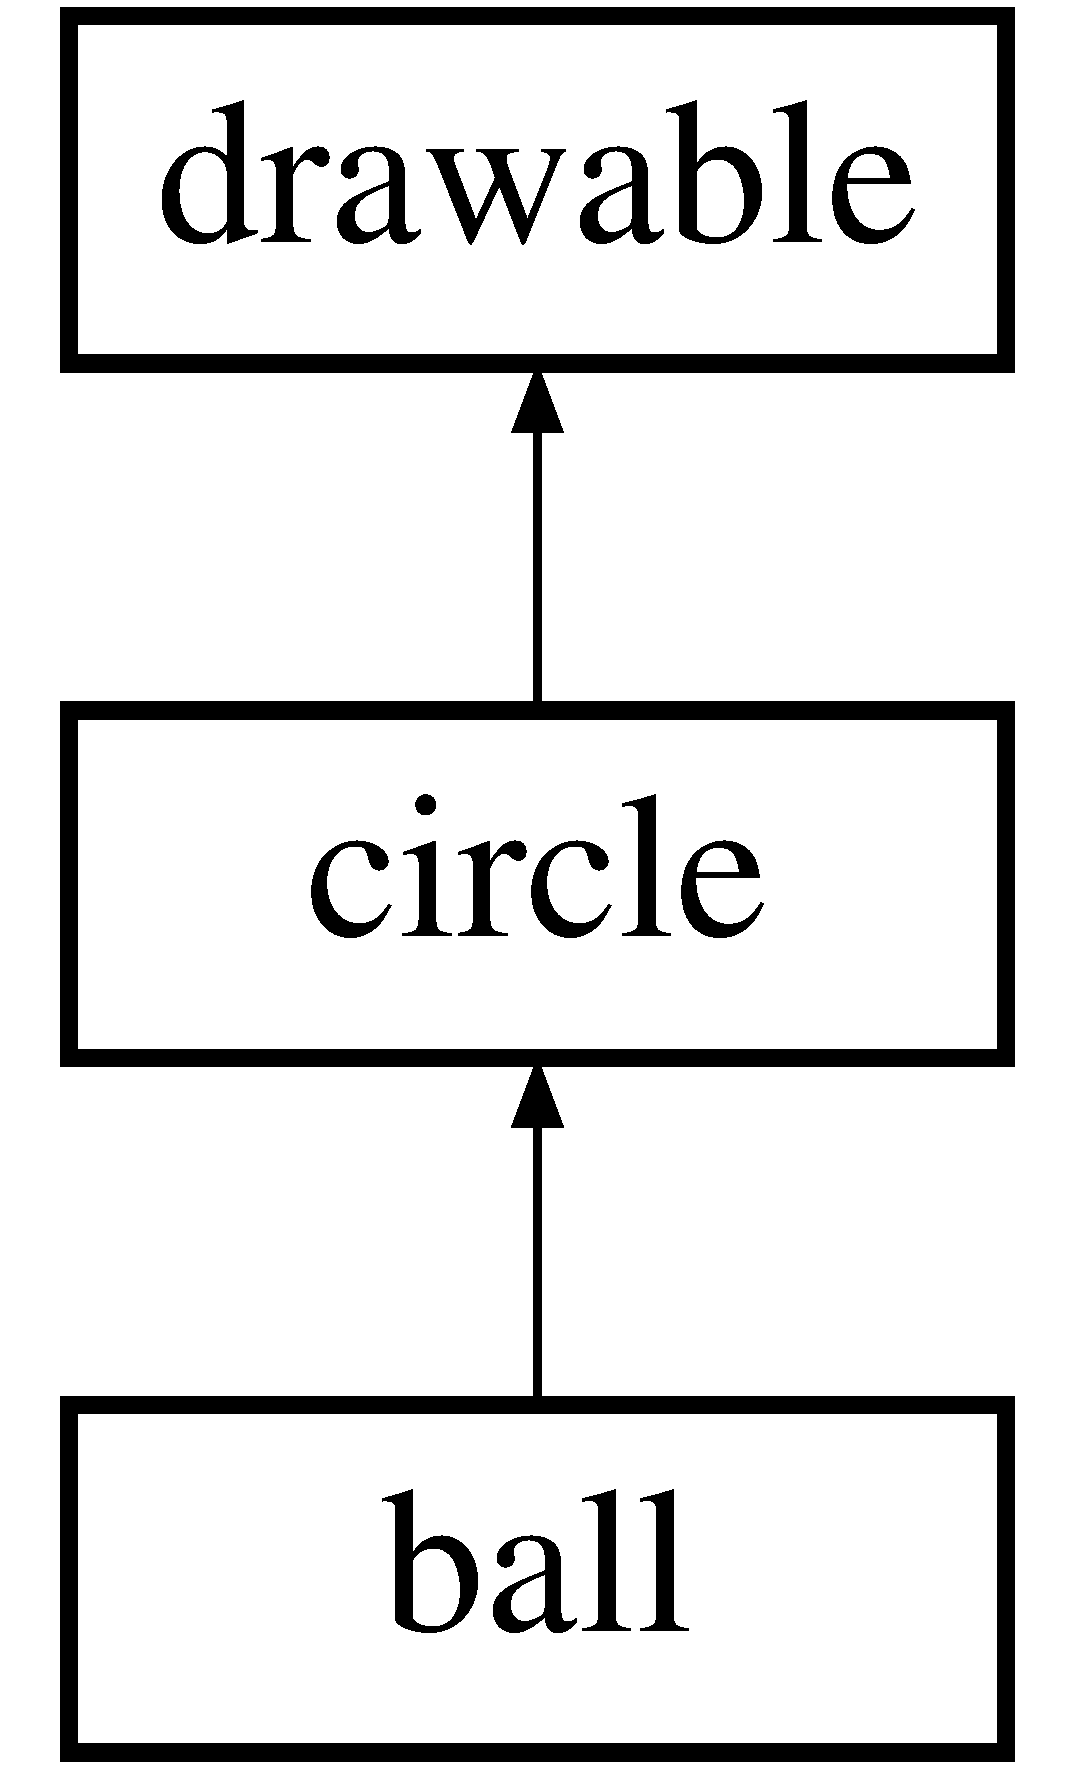
\includegraphics[height=3.000000cm]{classball}
\end{center}
\end{figure}
\subsection*{Public Member Functions}
\begin{DoxyCompactItemize}
\item 
\mbox{\Hypertarget{classball_a6fd1d27603e0ce43a922422fb651520e}\label{classball_a6fd1d27603e0ce43a922422fb651520e}} 
{\bfseries ball} (\hyperlink{classwindow}{window} \&w, const \hyperlink{classvector}{vector} \&midpoint, int radius, const \hyperlink{classvector}{vector} \&speed)
\item 
\mbox{\Hypertarget{classball_a5f291c177cdb80ae8d7c1f9328edbc6e}\label{classball_a5f291c177cdb80ae8d7c1f9328edbc6e}} 
void {\bfseries update} () override
\item 
\mbox{\Hypertarget{classball_a719362bf5934da38138a65693c02a593}\label{classball_a719362bf5934da38138a65693c02a593}} 
void {\bfseries interact} (\hyperlink{classdrawable}{drawable} \&other) override
\end{DoxyCompactItemize}
\subsection*{Additional Inherited Members}


The documentation for this class was generated from the following files\+:\begin{DoxyCompactItemize}
\item 
ball.\+hpp\item 
ball.\+cpp\end{DoxyCompactItemize}

\hypertarget{classcircle}{}\section{circle Class Reference}
\label{classcircle}\index{circle@{circle}}
\subsection*{Public Member Functions}
\begin{DoxyCompactItemize}
\item 
\mbox{\Hypertarget{classcircle_ac6ef4a49c741dcf33e5cf5d05768b450}\label{classcircle_ac6ef4a49c741dcf33e5cf5d05768b450}} 
{\bfseries circle} (\hyperlink{classwindow}{window} \&w, int mid\+\_\+x, int mid\+\_\+y, int radius)
\item 
\mbox{\Hypertarget{classcircle_a0c7d327e326648c249e1ba5439d1a7fa}\label{classcircle_a0c7d327e326648c249e1ba5439d1a7fa}} 
void {\bfseries print} ()
\end{DoxyCompactItemize}


The documentation for this class was generated from the following files\+:\begin{DoxyCompactItemize}
\item 
circle.\+hpp\item 
circle.\+cpp\end{DoxyCompactItemize}

\hypertarget{classdrawable}{}\section{drawable Class Reference}
\label{classdrawable}\index{drawable@{drawable}}
Inheritance diagram for drawable\+:\begin{figure}[H]
\begin{center}
\leavevmode
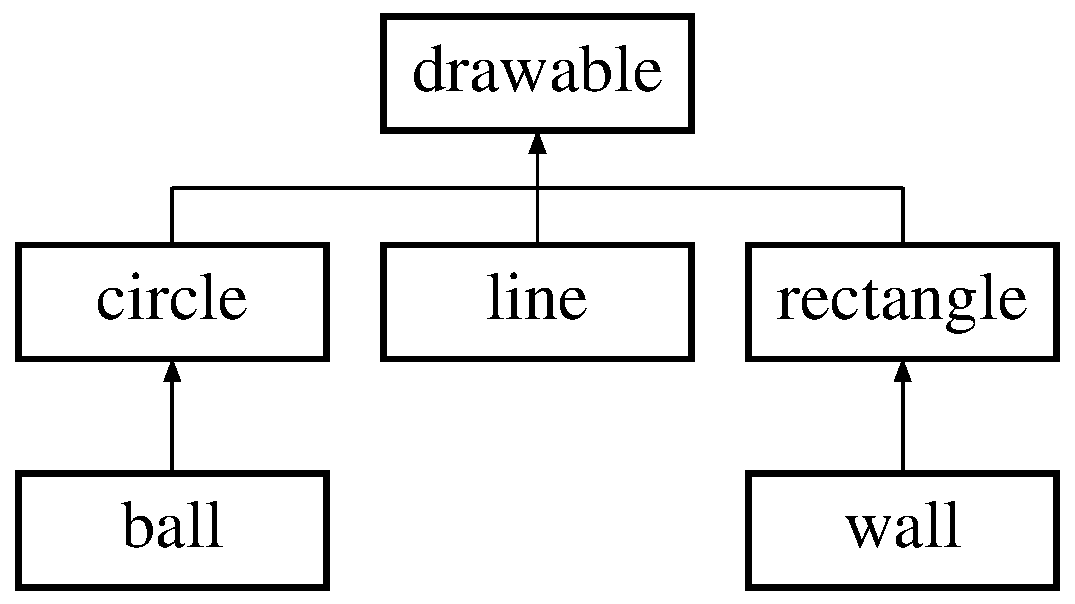
\includegraphics[height=3.000000cm]{classdrawable}
\end{center}
\end{figure}
\subsection*{Public Member Functions}
\begin{DoxyCompactItemize}
\item 
\mbox{\Hypertarget{classdrawable_a8fac7702c5f585c2d0deec8fb1fcc202}\label{classdrawable_a8fac7702c5f585c2d0deec8fb1fcc202}} 
{\bfseries drawable} (\hyperlink{classwindow}{window} \&w, const \hyperlink{classvector}{vector} \&location, const \hyperlink{classvector}{vector} \&size)
\item 
\mbox{\Hypertarget{classdrawable_a597f96aa3ae294757d9816c741cfc00a}\label{classdrawable_a597f96aa3ae294757d9816c741cfc00a}} 
bool {\bfseries overlaps} (const \hyperlink{classdrawable}{drawable} \&other)
\item 
\mbox{\Hypertarget{classdrawable_a5462dc7c98484f05fcaa4e30a55e953a}\label{classdrawable_a5462dc7c98484f05fcaa4e30a55e953a}} 
virtual void {\bfseries draw} ()=0
\item 
\mbox{\Hypertarget{classdrawable_a483266f1539329edc7e9ffa5068cdca7}\label{classdrawable_a483266f1539329edc7e9ffa5068cdca7}} 
virtual void {\bfseries update} ()
\item 
\mbox{\Hypertarget{classdrawable_ac36f995bf614accb3381db74e5f2b030}\label{classdrawable_ac36f995bf614accb3381db74e5f2b030}} 
virtual void {\bfseries interact} (\hyperlink{classdrawable}{drawable} \&other)
\item 
\mbox{\Hypertarget{classdrawable_a08bfd6356d7ab7bbe40c1e382dfbeda2}\label{classdrawable_a08bfd6356d7ab7bbe40c1e382dfbeda2}} 
std\+::ostream \& {\bfseries print} (std\+::ostream \&out) const
\end{DoxyCompactItemize}
\subsection*{Protected Attributes}
\begin{DoxyCompactItemize}
\item 
\mbox{\Hypertarget{classdrawable_a74aa041db41174597299018067370a03}\label{classdrawable_a74aa041db41174597299018067370a03}} 
\hyperlink{classwindow}{window} {\bfseries w}
\item 
\mbox{\Hypertarget{classdrawable_a7bff9c348bd2786022360c144f6a4212}\label{classdrawable_a7bff9c348bd2786022360c144f6a4212}} 
\hyperlink{classvector}{vector} {\bfseries location}
\item 
\mbox{\Hypertarget{classdrawable_aade7fdbfa85d4d5d737777451e6593e9}\label{classdrawable_aade7fdbfa85d4d5d737777451e6593e9}} 
\hyperlink{classvector}{vector} {\bfseries size}
\end{DoxyCompactItemize}


The documentation for this class was generated from the following files\+:\begin{DoxyCompactItemize}
\item 
drawable.\+hpp\item 
drawable.\+cpp\end{DoxyCompactItemize}

\hypertarget{classline}{}\section{line Class Reference}
\label{classline}\index{line@{line}}
Inheritance diagram for line\+:\begin{figure}[H]
\begin{center}
\leavevmode
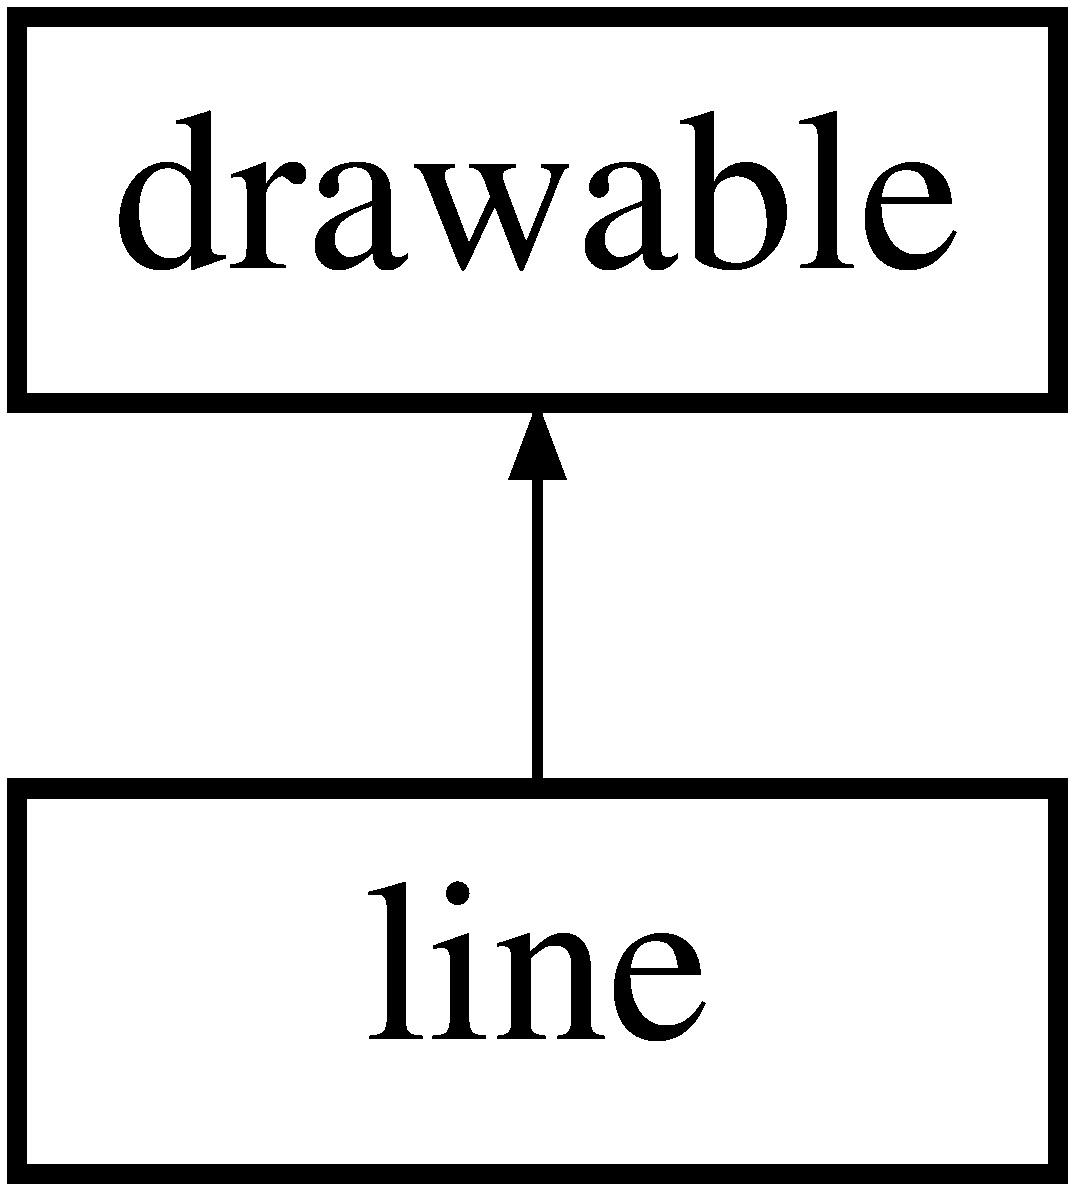
\includegraphics[height=2.000000cm]{classline}
\end{center}
\end{figure}
\subsection*{Public Member Functions}
\begin{DoxyCompactItemize}
\item 
\mbox{\Hypertarget{classline_a43ea2acfb458b795c9958508dadd9d18}\label{classline_a43ea2acfb458b795c9958508dadd9d18}} 
{\bfseries line} (\hyperlink{classwindow}{window} \&w, const \hyperlink{classvector}{vector} \&location, const \hyperlink{classvector}{vector} \&end)
\item 
\mbox{\Hypertarget{classline_af667c8ab35370df5d90e595cfb647c72}\label{classline_af667c8ab35370df5d90e595cfb647c72}} 
void {\bfseries draw} () override
\end{DoxyCompactItemize}
\subsection*{Additional Inherited Members}


The documentation for this class was generated from the following files\+:\begin{DoxyCompactItemize}
\item 
line.\+hpp\item 
line.\+cpp\end{DoxyCompactItemize}

\hypertarget{classrectangle}{}\section{rectangle Class Reference}
\label{classrectangle}\index{rectangle@{rectangle}}
Inheritance diagram for rectangle\+:\begin{figure}[H]
\begin{center}
\leavevmode
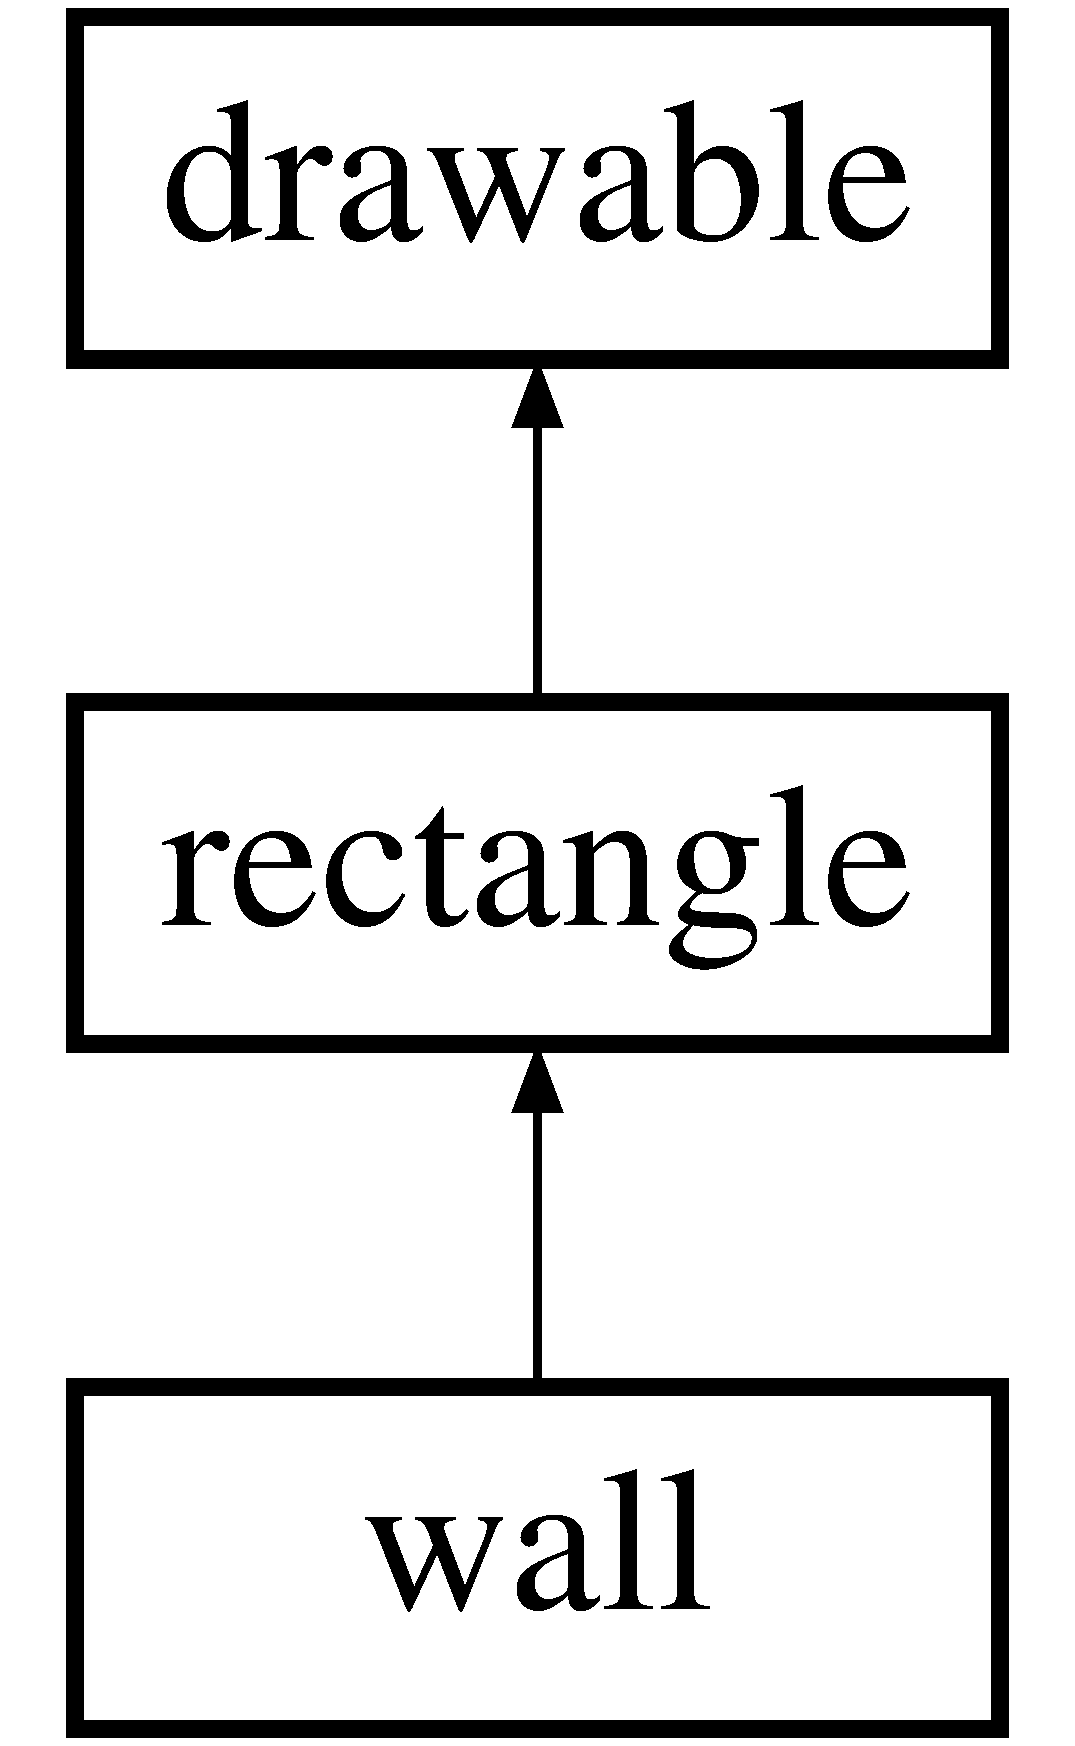
\includegraphics[height=3.000000cm]{classrectangle}
\end{center}
\end{figure}
\subsection*{Public Member Functions}
\begin{DoxyCompactItemize}
\item 
\mbox{\Hypertarget{classrectangle_a9e1157862932af46e234414c0bb56917}\label{classrectangle_a9e1157862932af46e234414c0bb56917}} 
{\bfseries rectangle} (\hyperlink{classwindow}{window} \&w, const \hyperlink{classvector}{vector} \&start, const \hyperlink{classvector}{vector} \&end)
\item 
\mbox{\Hypertarget{classrectangle_a5337a6fe8058087413729c523aadd65d}\label{classrectangle_a5337a6fe8058087413729c523aadd65d}} 
void {\bfseries draw} () override
\end{DoxyCompactItemize}
\subsection*{Protected Attributes}
\begin{DoxyCompactItemize}
\item 
\mbox{\Hypertarget{classrectangle_aee701f2f5c4d8dc8780ba9fac0693ac7}\label{classrectangle_aee701f2f5c4d8dc8780ba9fac0693ac7}} 
\hyperlink{classvector}{vector} {\bfseries end}
\item 
\mbox{\Hypertarget{classrectangle_a21aafb055b61a9b26b03a309a80b49c9}\label{classrectangle_a21aafb055b61a9b26b03a309a80b49c9}} 
\hyperlink{classvector}{vector} {\bfseries start}
\item 
\mbox{\Hypertarget{classrectangle_a76aa7276edfddfac8278d8d614686616}\label{classrectangle_a76aa7276edfddfac8278d8d614686616}} 
\hyperlink{classline}{line} {\bfseries left}
\item 
\mbox{\Hypertarget{classrectangle_a42d651a2358b3f91c47db91f7cd8878a}\label{classrectangle_a42d651a2358b3f91c47db91f7cd8878a}} 
\hyperlink{classline}{line} {\bfseries right}
\item 
\mbox{\Hypertarget{classrectangle_a91b67581c0120705272c701cdc4bb716}\label{classrectangle_a91b67581c0120705272c701cdc4bb716}} 
\hyperlink{classline}{line} {\bfseries top}
\item 
\mbox{\Hypertarget{classrectangle_a356858f50aa3f38731f62bc7aa57dfad}\label{classrectangle_a356858f50aa3f38731f62bc7aa57dfad}} 
\hyperlink{classline}{line} {\bfseries bottom}
\end{DoxyCompactItemize}


The documentation for this class was generated from the following files\+:\begin{DoxyCompactItemize}
\item 
rectangle.\+hpp\item 
rectangle.\+cpp\end{DoxyCompactItemize}

\hypertarget{classvector}{}\section{vector Class Reference}
\label{classvector}\index{vector@{vector}}


vector operator  




{\ttfamily \#include $<$vector.\+hpp$>$}

\subsection*{Public Member Functions}
\begin{DoxyCompactItemize}
\item 
\hyperlink{classvector_ada69c108ec9393e6f70bdfcd58366cbf}{vector} (int x=0, int y=0)
\begin{DoxyCompactList}\small\item\em The constructor of an Vector. \end{DoxyCompactList}\item 
\hyperlink{classvector}{vector} \hyperlink{classvector_a9af16b41f973cd073b089bf5371e8a70}{operator+} () const
\begin{DoxyCompactList}\small\item\em returns himself vector \end{DoxyCompactList}\item 
\hyperlink{classvector}{vector} \hyperlink{classvector_a9d639bc53d77f17c6ba3af1dd9549424}{operator+} (const \hyperlink{classvector}{vector} \&rhs) const
\begin{DoxyCompactList}\small\item\em Adds 2 vector into a new vector. \end{DoxyCompactList}\item 
\hyperlink{classvector}{vector} \& \hyperlink{classvector_a401c12597814627f350a8cd663b6dba5}{operator+=} (const \hyperlink{classvector}{vector} \&rhs)
\begin{DoxyCompactList}\small\item\em Adds a vector into another vector. \end{DoxyCompactList}\item 
bool \hyperlink{classvector_a0066b879f704f7d344ec9cd2a2f57ea3}{operator==} (const \hyperlink{classvector}{vector} \&rhs) const
\begin{DoxyCompactList}\small\item\em Compares 2 vectors. \end{DoxyCompactList}\item 
\hyperlink{classvector}{vector} \hyperlink{classvector_ad4e924ee21af1367f8724b2d94db110e}{operator$\ast$} (const int rhs) const
\begin{DoxyCompactList}\small\item\em multiplies a vector with an integer \end{DoxyCompactList}\item 
\hyperlink{classvector}{vector} \hyperlink{classvector_a9ef97fde561d0998f1db1af7c9fbbff8}{operator$\ast$} (const \hyperlink{classvector}{vector} \&rhs) const
\begin{DoxyCompactList}\small\item\em multiplies 2 vectors \end{DoxyCompactList}\item 
\hyperlink{classvector}{vector} \& \hyperlink{classvector_ad7dba928c0f8e3bef217dd1d97ebfb8f}{operator$\ast$=} (const \hyperlink{classvector}{vector} \&rhs)
\begin{DoxyCompactList}\small\item\em multiplies a vector into a vector \end{DoxyCompactList}\end{DoxyCompactItemize}
\subsection*{Public Attributes}
\begin{DoxyCompactItemize}
\item 
\mbox{\Hypertarget{classvector_a0403eb3aea23a3009e276fba1d317046}\label{classvector_a0403eb3aea23a3009e276fba1d317046}} 
int {\bfseries x}
\item 
\mbox{\Hypertarget{classvector_aad6de640298eae97ca0a094db5aff477}\label{classvector_aad6de640298eae97ca0a094db5aff477}} 
int {\bfseries y}
\end{DoxyCompactItemize}
\subsection*{Friends}
\begin{DoxyCompactItemize}
\item 
std\+::ostream \& \hyperlink{classvector_a7a6813f75dabd6f9575f9d6f91890255}{operator$<$$<$} (std\+::ostream \&lhs, const \hyperlink{classvector}{vector} \&rhs)
\begin{DoxyCompactList}\small\item\em prints a vector in the command line \end{DoxyCompactList}\end{DoxyCompactItemize}


\subsection{Detailed Description}
vector operator 

this library contains a c++ and a h++ file, it defines and declares some operator, used with a vector. it also contains a constructor for a vector 

\subsection{Constructor \& Destructor Documentation}
\mbox{\Hypertarget{classvector_ada69c108ec9393e6f70bdfcd58366cbf}\label{classvector_ada69c108ec9393e6f70bdfcd58366cbf}} 
\index{vector@{vector}!vector@{vector}}
\index{vector@{vector}!vector@{vector}}
\subsubsection{\texorpdfstring{vector()}{vector()}}
{\footnotesize\ttfamily vector\+::vector (\begin{DoxyParamCaption}\item[{int}]{x = {\ttfamily 0},  }\item[{int}]{y = {\ttfamily 0} }\end{DoxyParamCaption})}



The constructor of an Vector. 

This is a constructor that makes a vector from two parameters a x pos and a y pos, with a default value of 0 for both pos 

\subsection{Member Function Documentation}
\mbox{\Hypertarget{classvector_ad4e924ee21af1367f8724b2d94db110e}\label{classvector_ad4e924ee21af1367f8724b2d94db110e}} 
\index{vector@{vector}!operator$\ast$@{operator$\ast$}}
\index{operator$\ast$@{operator$\ast$}!vector@{vector}}
\subsubsection{\texorpdfstring{operator$\ast$()}{operator*()}\hspace{0.1cm}{\footnotesize\ttfamily [1/2]}}
{\footnotesize\ttfamily \hyperlink{classvector}{vector} vector\+::operator$\ast$ (\begin{DoxyParamCaption}\item[{const int}]{rhs }\end{DoxyParamCaption}) const}



multiplies a vector with an integer 

This operator multiplies a vector with an integer into a new vector, the new vector is returned \mbox{\Hypertarget{classvector_a9ef97fde561d0998f1db1af7c9fbbff8}\label{classvector_a9ef97fde561d0998f1db1af7c9fbbff8}} 
\index{vector@{vector}!operator$\ast$@{operator$\ast$}}
\index{operator$\ast$@{operator$\ast$}!vector@{vector}}
\subsubsection{\texorpdfstring{operator$\ast$()}{operator*()}\hspace{0.1cm}{\footnotesize\ttfamily [2/2]}}
{\footnotesize\ttfamily \hyperlink{classvector}{vector} vector\+::operator$\ast$ (\begin{DoxyParamCaption}\item[{const \hyperlink{classvector}{vector} \&}]{rhs }\end{DoxyParamCaption}) const}



multiplies 2 vectors 

This operator multiplies 2 vector into a new vector, the new vector is returned \mbox{\Hypertarget{classvector_ad7dba928c0f8e3bef217dd1d97ebfb8f}\label{classvector_ad7dba928c0f8e3bef217dd1d97ebfb8f}} 
\index{vector@{vector}!operator$\ast$=@{operator$\ast$=}}
\index{operator$\ast$=@{operator$\ast$=}!vector@{vector}}
\subsubsection{\texorpdfstring{operator$\ast$=()}{operator*=()}}
{\footnotesize\ttfamily \hyperlink{classvector}{vector} \& vector\+::operator$\ast$= (\begin{DoxyParamCaption}\item[{const \hyperlink{classvector}{vector} \&}]{rhs }\end{DoxyParamCaption})}



multiplies a vector into a vector 

This operator multiplies a vector into a vector, thereby it changes the first vector the first vector is returned \mbox{\Hypertarget{classvector_a9af16b41f973cd073b089bf5371e8a70}\label{classvector_a9af16b41f973cd073b089bf5371e8a70}} 
\index{vector@{vector}!operator+@{operator+}}
\index{operator+@{operator+}!vector@{vector}}
\subsubsection{\texorpdfstring{operator+()}{operator+()}\hspace{0.1cm}{\footnotesize\ttfamily [1/2]}}
{\footnotesize\ttfamily \hyperlink{classvector}{vector} vector\+::operator+ (\begin{DoxyParamCaption}{ }\end{DoxyParamCaption}) const}



returns himself vector 

This operatotor return himself \mbox{\Hypertarget{classvector_a9d639bc53d77f17c6ba3af1dd9549424}\label{classvector_a9d639bc53d77f17c6ba3af1dd9549424}} 
\index{vector@{vector}!operator+@{operator+}}
\index{operator+@{operator+}!vector@{vector}}
\subsubsection{\texorpdfstring{operator+()}{operator+()}\hspace{0.1cm}{\footnotesize\ttfamily [2/2]}}
{\footnotesize\ttfamily \hyperlink{classvector}{vector} vector\+::operator+ (\begin{DoxyParamCaption}\item[{const \hyperlink{classvector}{vector} \&}]{rhs }\end{DoxyParamCaption}) const}



Adds 2 vector into a new vector. 

This operator return a vector made from adding the x\+\_\+pos and the y\+\_\+pos of both vector \mbox{\Hypertarget{classvector_a401c12597814627f350a8cd663b6dba5}\label{classvector_a401c12597814627f350a8cd663b6dba5}} 
\index{vector@{vector}!operator+=@{operator+=}}
\index{operator+=@{operator+=}!vector@{vector}}
\subsubsection{\texorpdfstring{operator+=()}{operator+=()}}
{\footnotesize\ttfamily \hyperlink{classvector}{vector} \& vector\+::operator+= (\begin{DoxyParamCaption}\item[{const \hyperlink{classvector}{vector} \&}]{rhs }\end{DoxyParamCaption})}



Adds a vector into another vector. 

This operator adds a vector into another vector Thereby it changes the first vector and returns himself \mbox{\Hypertarget{classvector_a0066b879f704f7d344ec9cd2a2f57ea3}\label{classvector_a0066b879f704f7d344ec9cd2a2f57ea3}} 
\index{vector@{vector}!operator==@{operator==}}
\index{operator==@{operator==}!vector@{vector}}
\subsubsection{\texorpdfstring{operator==()}{operator==()}}
{\footnotesize\ttfamily bool vector\+::operator== (\begin{DoxyParamCaption}\item[{const \hyperlink{classvector}{vector} \&}]{rhs }\end{DoxyParamCaption}) const}



Compares 2 vectors. 

This operator compares 2 vectors there x\+\_\+pos and y\+\_\+pos and returns a boo value 

\subsection{Friends And Related Function Documentation}
\mbox{\Hypertarget{classvector_a7a6813f75dabd6f9575f9d6f91890255}\label{classvector_a7a6813f75dabd6f9575f9d6f91890255}} 
\index{vector@{vector}!operator$<$$<$@{operator$<$$<$}}
\index{operator$<$$<$@{operator$<$$<$}!vector@{vector}}
\subsubsection{\texorpdfstring{operator$<$$<$}{operator<<}}
{\footnotesize\ttfamily std\+::ostream\& operator$<$$<$ (\begin{DoxyParamCaption}\item[{std\+::ostream \&}]{lhs,  }\item[{const \hyperlink{classvector}{vector} \&}]{rhs }\end{DoxyParamCaption})\hspace{0.3cm}{\ttfamily [friend]}}



prints a vector in the command line 

This operator prints a into the command line 

The documentation for this class was generated from the following files\+:\begin{DoxyCompactItemize}
\item 
\hyperlink{vector_8hpp}{vector.\+hpp}\item 
vector.\+cpp\end{DoxyCompactItemize}

\hypertarget{classwall}{}\section{wall Class Reference}
\label{classwall}\index{wall@{wall}}


wall  




{\ttfamily \#include $<$wall.\+hpp$>$}

Inheritance diagram for wall\+:\begin{figure}[H]
\begin{center}
\leavevmode
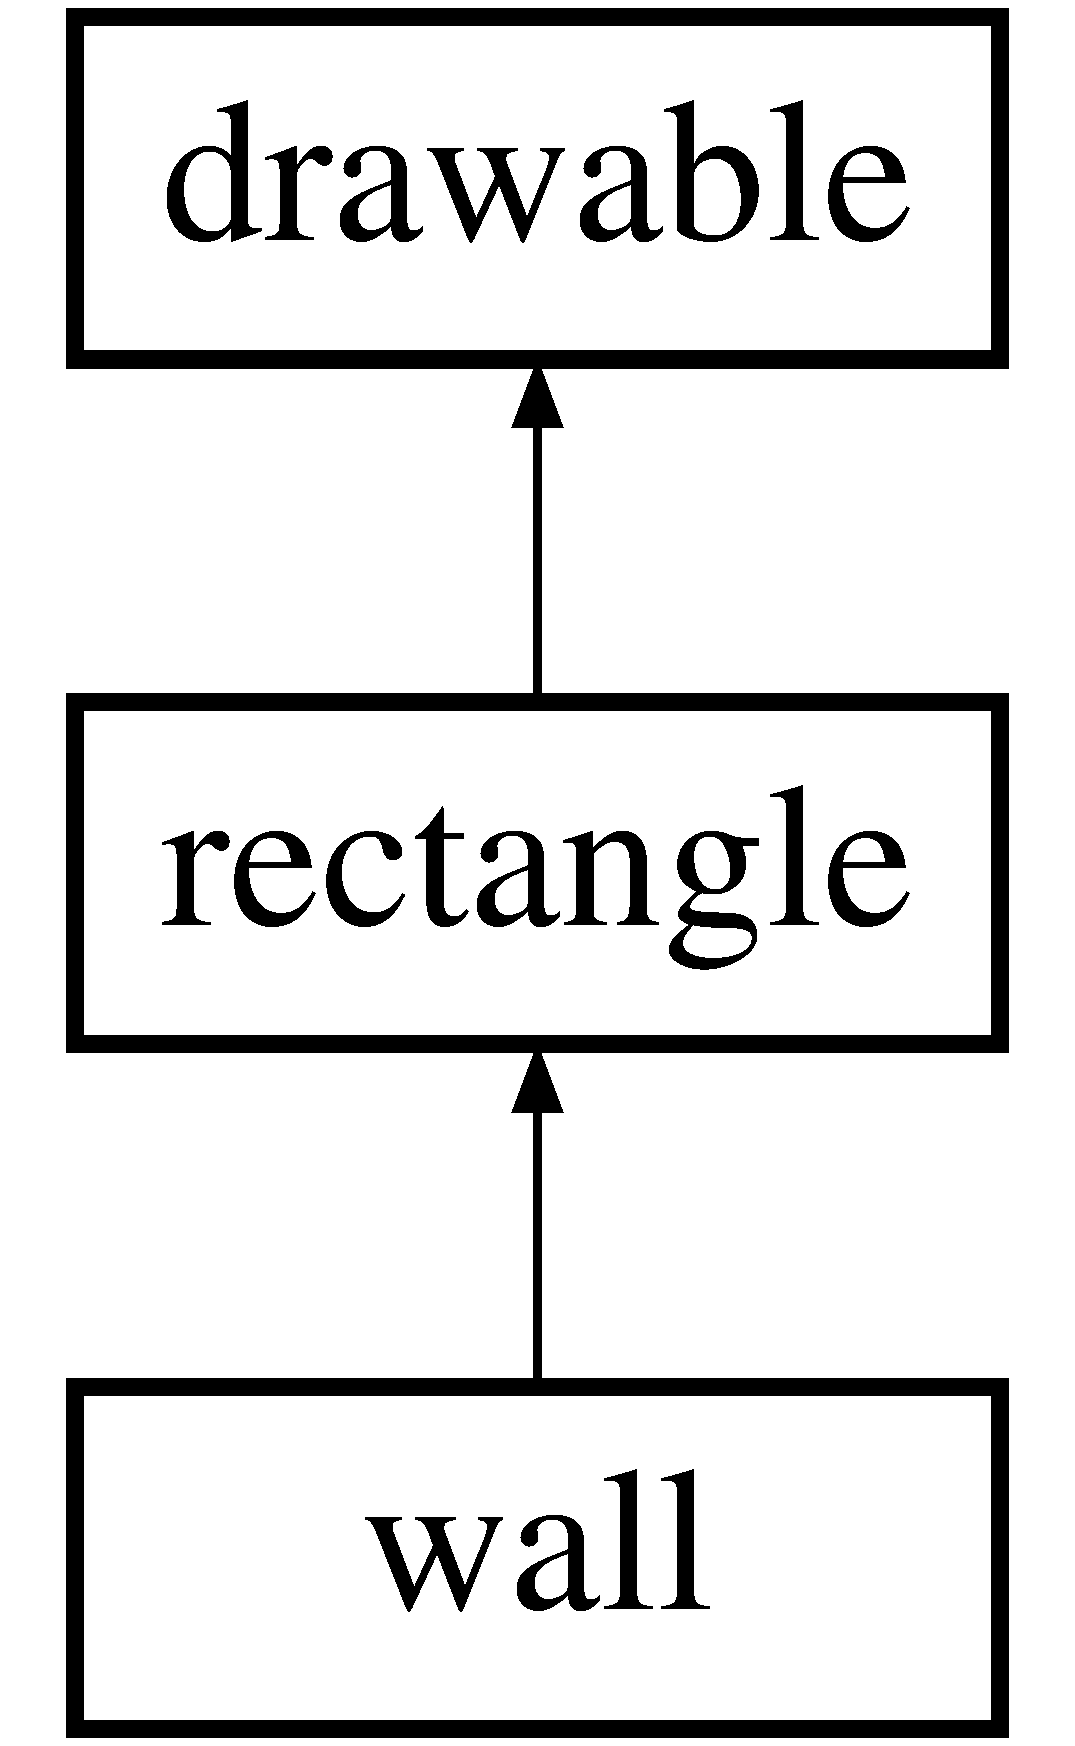
\includegraphics[height=3.000000cm]{classwall}
\end{center}
\end{figure}
\subsection*{Public Member Functions}
\begin{DoxyCompactItemize}
\item 
\hyperlink{classwall_a6bbd0a74571562b849a2446ba29978dc}{wall} (\hyperlink{classwindow}{window} \&w, const \hyperlink{classvector}{vector} \&start, const \hyperlink{classvector}{vector} \&end, int update\+\_\+interval)
\begin{DoxyCompactList}\small\item\em The constructor of a wall. \end{DoxyCompactList}\item 
void \hyperlink{classwall_abbae6802729e5a2e2a83a61694747b33}{draw} () override
\begin{DoxyCompactList}\small\item\em a draw function of a wall \end{DoxyCompactList}\item 
void \hyperlink{classwall_a84c4981162efc4f914e064c30ad52f03}{update} () override
\begin{DoxyCompactList}\small\item\em a update function of a wall \end{DoxyCompactList}\end{DoxyCompactItemize}
\subsection*{Protected Attributes}
\begin{DoxyCompactItemize}
\item 
\mbox{\Hypertarget{classwall_a2af7171cd8c999284e9ebdd7eac8cfea}\label{classwall_a2af7171cd8c999284e9ebdd7eac8cfea}} 
bool {\bfseries filled}
\item 
\mbox{\Hypertarget{classwall_ab3bc2d0218d9c5b24969f74571bc9b96}\label{classwall_ab3bc2d0218d9c5b24969f74571bc9b96}} 
int {\bfseries update\+\_\+interval}
\item 
\mbox{\Hypertarget{classwall_abaaa1fcf2ab29e7c4523b6526ad03f2f}\label{classwall_abaaa1fcf2ab29e7c4523b6526ad03f2f}} 
int {\bfseries update\+\_\+count}
\end{DoxyCompactItemize}


\subsection{Detailed Description}
wall 

this library contains a c++ and a h++ file, it contains a constructor, a draw function and a update function 

\subsection{Constructor \& Destructor Documentation}
\mbox{\Hypertarget{classwall_a6bbd0a74571562b849a2446ba29978dc}\label{classwall_a6bbd0a74571562b849a2446ba29978dc}} 
\index{wall@{wall}!wall@{wall}}
\index{wall@{wall}!wall@{wall}}
\subsubsection{\texorpdfstring{wall()}{wall()}}
{\footnotesize\ttfamily wall\+::wall (\begin{DoxyParamCaption}\item[{\hyperlink{classwindow}{window} \&}]{w,  }\item[{const \hyperlink{classvector}{vector} \&}]{start,  }\item[{const \hyperlink{classvector}{vector} \&}]{end,  }\item[{int}]{update\+\_\+interval }\end{DoxyParamCaption})}



The constructor of a wall. 

This is a constructor that makes a wall from four parameters it has a start and an end pos also an update interval 

\subsection{Member Function Documentation}
\mbox{\Hypertarget{classwall_abbae6802729e5a2e2a83a61694747b33}\label{classwall_abbae6802729e5a2e2a83a61694747b33}} 
\index{wall@{wall}!draw@{draw}}
\index{draw@{draw}!wall@{wall}}
\subsubsection{\texorpdfstring{draw()}{draw()}}
{\footnotesize\ttfamily void wall\+::draw (\begin{DoxyParamCaption}{ }\end{DoxyParamCaption})\hspace{0.3cm}{\ttfamily [override]}, {\ttfamily [virtual]}}



a draw function of a wall 

if filled this function makes a wall using 4 rectangles, each an pixel thick 

Reimplemented from \hyperlink{classrectangle}{rectangle}.

\mbox{\Hypertarget{classwall_a84c4981162efc4f914e064c30ad52f03}\label{classwall_a84c4981162efc4f914e064c30ad52f03}} 
\index{wall@{wall}!update@{update}}
\index{update@{update}!wall@{wall}}
\subsubsection{\texorpdfstring{update()}{update()}}
{\footnotesize\ttfamily void wall\+::update (\begin{DoxyParamCaption}{ }\end{DoxyParamCaption})\hspace{0.3cm}{\ttfamily [override]}, {\ttfamily [virtual]}}



a update function of a wall 

this count towards the update counts, if meeted it inverts the state of filled 

Reimplemented from \hyperlink{classdrawable}{drawable}.



The documentation for this class was generated from the following files\+:\begin{DoxyCompactItemize}
\item 
\hyperlink{wall_8hpp}{wall.\+hpp}\item 
wall.\+cpp\end{DoxyCompactItemize}

\hypertarget{classwindow}{}\section{window Class Reference}
\label{classwindow}\index{window@{window}}
\subsection*{Public Member Functions}
\begin{DoxyCompactItemize}
\item 
\mbox{\Hypertarget{classwindow_a26b54741901955b42941d3e08f09ba83}\label{classwindow_a26b54741901955b42941d3e08f09ba83}} 
{\bfseries window} (int x\+\_\+size, int y\+\_\+size, int scale)
\item 
\mbox{\Hypertarget{classwindow_a20541f9e1801404baf9a9184365e9b93}\label{classwindow_a20541f9e1801404baf9a9184365e9b93}} 
void {\bfseries draw} (int x, int y)
\item 
\mbox{\Hypertarget{classwindow_a6c050475db28a9b773cf2edbc56ece86}\label{classwindow_a6c050475db28a9b773cf2edbc56ece86}} 
void {\bfseries clear} ()
\end{DoxyCompactItemize}


The documentation for this class was generated from the following files\+:\begin{DoxyCompactItemize}
\item 
window.\+hpp\item 
window.\+cpp\end{DoxyCompactItemize}

\chapter{File Documentation}
\hypertarget{wall_8hpp}{}\section{wall.\+hpp File Reference}
\label{wall_8hpp}\index{wall.\+hpp@{wall.\+hpp}}
{\ttfamily \#include \char`\"{}window.\+hpp\char`\"{}}\newline
{\ttfamily \#include \char`\"{}drawable.\+hpp\char`\"{}}\newline
{\ttfamily \#include \char`\"{}vector.\+hpp\char`\"{}}\newline
{\ttfamily \#include \char`\"{}line.\+hpp\char`\"{}}\newline
{\ttfamily \#include \char`\"{}rectangle.\+hpp\char`\"{}}\newline
\subsection*{Classes}
\begin{DoxyCompactItemize}
\item 
class \hyperlink{classwall}{wall}
\begin{DoxyCompactList}\small\item\em wall \end{DoxyCompactList}\end{DoxyCompactItemize}

%--- End generated contents ---

% Index
\backmatter
\newpage
\phantomsection
\clearemptydoublepage
\addcontentsline{toc}{chapter}{Index}
\printindex

\end{document}
